\subsection{System}
Ein System besteht aus mehreren Einzelgeräten, mit welchen, wie vorhin beschrieben, das Zählen, die Kategorisierung und die Geschwindigkeitsmessung durchgeführt wird. Es werden mehrere Geräte benötigt, um den Verkehrsfluss im definiert begrenzten Gebiet darstellen zu können. Dabei konnte der Verkehrsfluss mithilfe des aufgenommenen Zeitstempels und der Fahrtrichtung statistisch rekonstruiert werden. Hierbei konnte das vorhin erstellte Netzwerk des begrenzten Gebietes, als Darstellungsgrundlage verwendet werden. Zunächst wurden die nächstgelegenen Geräte, welche auf direktem Weg erreichbar sind, identifiziert und von diesen die Daten des Feature Vektors extrahiert. Diese Daten wurden dann nach dem Zeitstempel sortiert und mit einem Index versehen. Nachdem die Daten vorbereitet waren, wurde die voraussichtliche Durchfahrtszeit anhand der Abstände der Geräte anhand einer Testmessung bestimmt. Wenn die Verkehrsteilnehmer die Geschwindigkeitsbegrenzungen einhalten, dan brauchen diese die Zeiten welche unten in \tref{tFahrzeiten}  aufgelistet sind. Die höchste Wahrscheinlichkeit, welchen Weg der Verkehrsteilnehmer nahm, konnte aufgrund dessen berechnet und anschliessened eingezeichnet werden. Der geschilderte Vorgang konnte mit jedem Geräte durchgeführt und diese untereinander verglichen werden. Die möglichen Wege wurden dem Netzwerk ergänzt und somit konnte die folgende Auswertung (\fref{bAuswertung}) durchgeführt werden.\\\\

\begin{table}[H]
\centering
    \begin{tabular}{p{5cm}l}
    \textbf{Fahrtweg}                & \textbf{Zeit in Sekunden}   \\
    1 nach 2                           & 60  \\
    1 nach 3		                   & 50  \\
    2 nach 3	                       & 60  \\ 
    2 nach 4	                       & 100 \\
    2 nach 5                           & 85  \\
    2 nach 6                   		   & 70  \\
    4 nach 5                   		   & 80  \\
    4 nach 6                   		   & 150 \\
    5 nach 6                   		   & 140 \\   
\end{tabular}
\caption{Fahrzeiten zwischen den Stationen}
\label{tFahrzeiten}
\end{table}

\begin{figure}[H]
  \centering
  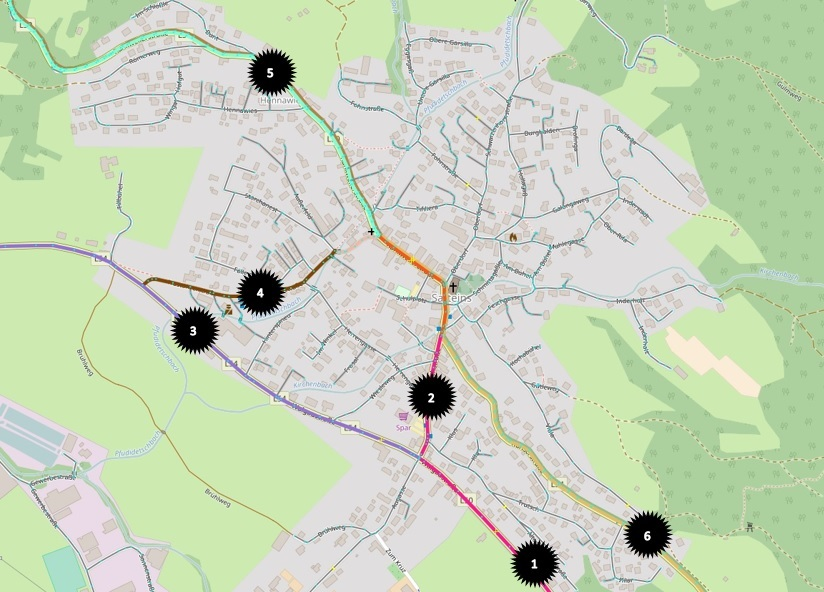
\includegraphics[width=0.6\textwidth]{Resultate/Auswertung.jpg} 
  \caption{Darstellung des Verkehrsflusses in Satteins.}
  \label{bAuswertung}
\end{figure}
In \tref{tVerkehrsfluss} ist der Verkehrsfluss von jedem Gerät zu seinem direkten Nachfolger tabellarisch dargestellt. 

\setlength\tabcolsep{5pt}

\begin{table}[H]
\centering
\begin{tabular}{|p{1.5cm}|p{1.5cm}|p{1.5cm}|p{1.5cm}|p{1.5cm}|p{1.5cm}|p{1.5cm}|p{1.5cm}|}
\hline
	von/nach & 1 & 2 & 3 & 4 & 5 & 6 & Out \\ \hline
	1 &  & 952 & 849 &  &  &  & 1874 \\ \hline
	2 & 926 &  & 679 & 105 & 834 & 575 &  \\ \hline
	3 & 996 & 852 &  &  & &  & 1719 \\ \hline
	4 &  & 149 &  &  & 105 & 84 & 520 \\ \hline
	5 &  & 723 &  & 159 & 521 & 224 & 1668 \\ \hline
	6 &  & 313 &  & 78 & 326 &  & 720 \\ \hline
\end{tabular}
\caption{Tabelarische Darstellung des Verkehrsflusses.}
\label{tVerkehrsfluss}
\end{table}
\setlength\tabcolsep{0pt}

In der nachfolgenden Tabelle (\tref{tstVerkehr}) ist zu jeder Stunde, der vorbeifahrende Verkehr jedes Gerätes aufgetragen. Dabei wurden die vorbeifahrenden Fahrzeuge in folgende Fahrtrichtungen eingeteilt. "'Raus"' bedeutet, dass sich das Fahrzeug vom Ortszentrum weg bewegt hat. "'Rein"' heisst, dass es in Richtung Ortszentrum gefahrten ist.

\setlength\tabcolsep{5pt}
\begin{table}[H]
\centering
\begin{tabular}{|l|l|l|l|l|l|l|l|l|l|l|l|l|}
\hline
\textbf{Station}        & \multicolumn{2}{l|}{\textbf{1}}                 & \multicolumn{2}{l|}{\textbf{2}}                 & \multicolumn{2}{l|}{\textbf{3}}                 & \multicolumn{2}{l|}{\textbf{4}}               & \multicolumn{2}{l|}{\textbf{5}}                 & \multicolumn{2}{l|}{\textbf{6}}               \\ \hline
\textbf{Uhrzeit}        & Rein                   & Raus                   & Rein                   & Raus                   & Rein                   & Raus                   & Rein                  & Raus                  & Rein                   & Raus                   & Rein                  & Raus                  \\ \hline
\textbf{4-5}            & 28                     & 28                     & 24                     & 28                     & 59                     & 17                     & 3                     & 1                     & 20                     & 12                     & 22                    & 24                    \\ \hline
\textbf{5-6}            & 102                    & 105                    & 56                     & 71                     & 171                    & 51                     & 72                    & 20                    & 117                    & 84                     & 20                    & 67                    \\ \hline
\textbf{6-7}            & 173                    & 187                    & 84                     & 64                     & 218                    & 104                    & 57                    & 30                    & 190                    & 117                    & 29                    & 85                    \\ \hline
\textbf{7-8}            & 159                    & 98                     & 63                     & 103                    & 132                    & 86                     & 39                    & 16                    & 104                    & 80                     & 33                    & 50                    \\ \hline
\textbf{8-9}            & 88                     & 92                     & 160                    & 124                    & 95                     & 112                    & 21                    & 28                    & 79                     & 84                     & 23                    & 25                    \\ \hline
\textbf{9-10}           & 133                    & 155                    & 137                    & 87                     & 102                    & 98                     & 36                    & 36                    & 79                     & 118                    & 28                    & 48                    \\ \hline
\textbf{10-11}          & 110                    & 119                    & 233                    & 111                    & 115                    & 152                    & 19                    & 47                    & 84                     & 125                    & 40                    & 40                    \\ \hline
\textbf{11-12}          & 107                    & 151                    & 64                     & 114                    & 163                    & 183                    & 25                    & 48                    & 93                     & 108                    & 62                    & 74                    \\ \hline
\textbf{12-13}          & 178                    & 161                    & 168                    & 147                    & 102                    & 164                    & 31                    & 38                    & 106                    & 104                    & 33                    & 59                    \\ \hline
\textbf{13-14}          & 161                    & 117                    & 132                    & 134                    & 132                    & 112                    & 34                    & 58                    & 117                    & 126                    & 64                    & 61                    \\ \hline
\textbf{14-15}          & 120                    & 131                    & 165                    & 88                     & 89                     & 101                    & 12                    & 23                    & 54                     & 69                     & 46                    & 44                    \\ \hline
\textbf{15-16}          & 142                    & 165                    & 226                    & 173                    & 105                    & 126                    & 37                    & 50                    & 103                    & 182                    & 72                    & 42                    \\ \hline
\textbf{16-17}          & 178                    & 156                    & 156                    & 163                    & 75                     & 145                    & 25                    & 50                    & 116                    & 216                    & 93                    & 36                    \\ \hline
\textbf{17-18}          & 72                     & 80                     & 182                    & 86                     & 126                    & 78                     & 16                    & 35                    & 75                     & 105                    & 39                    & 20                    \\ \hline
\textbf{18-19}          & 58                     & 69                     & 156                    & 84                     & 76                     & 127                    & 33                    & 24                    & 47                     & 80                     & 32                    & 27                    \\ \hline
\textbf{19-20}          & 58                     & 60                     & 73                     & 40                     & 83                     & 63                     & 4                     & 16                    & 46                     & 58                     & 21                    & 18                    \\ \hline
\textit{\textbf{Total}} & \textit{\textbf{1867}} & \textit{\textbf{1874}} & \textit{\textbf{2079}} & \textit{\textbf{1617}} & \textit{\textbf{1843}} & \textit{\textbf{1719}} & \textit{\textbf{464}} & \textit{\textbf{520}} & \textit{\textbf{1430}} & \textit{\textbf{1668}} & \textit{\textbf{657}} & \textit{\textbf{720}} \\ \hline
\end{tabular}
\caption{Stündlicher Verkehr bei jeder Station.}
\label{tstVerkehr}
\end{table}
\setlength\tabcolsep{0pt}